\chapter{Motion Capture for a Natural Tree in the Wind} 
\label{chap:pilottree}

\noindent
Jie Long, Cory Reimschussel, Ontario Britton, and Michael Jones. Motion capture for natural tree animation. \emph{International Conference on Computer Graphics and Interactive Techniques, SIGGRAPH 2009: Talks}. New Orleans, Louisiana, Article No. 77, 2009.

\begin{abstract}
Simulating the motion of a tree in the wind is a difficult problem because of the complexity of the tree's geometry and its associated wind dynamics. Physically based animation of trees in the wind is computationally expensive, while noise-based approaches ignore important global effects, such as sheltering. Motion capture may help solve these problems. In this paper, we present new approaches to inferring a skeleton from tree motion data and repairing motion data using a rigid body model. While the rigid body model can be used to extract data, the data contains many gaps and errors for branches that bend. Motion data repair is critical because trees are not rigid bodies. These ideas allow the reconstruction of tree motion, including global effects, but without a complex physical model.
\end{abstract}

\section{Introduction}

We address the problem of animating natural trees in games with greater accuracy but without additional computational overhead compared to techniques based on velocity or force textures---such as \cite{Habel09PGT}. We believe that motion capture is one way to accomplish this goal. Motion capture of tree motion in the wind is difficult because the tree branching structure is both important and difficult to model and because branches are non-rigid bodies at large deflections.   

Accurate animation of trees is important to both CG animators and forestry ecologists. CG animators can use plausible and directable models of tree motion in digital storytelling.  In a game, trees moving in the wind can be used to emphasize weather or create a sense of foreboding. Forestry ecologists can use models of tree motion to design pruning methodologies that maximize yield while minimizing windthrow potential. 

Many approaches have been taken to modeling tree structure and geometry. Recent photo-based approaches to tree modeling \cite{neubert:acmtg07,RecheMartinez2004,Tan:2007:ITM} are particularly relevant to this work. Photo-based methods plausibly recreate 3D natural tree models by approximating the branching structure of photographed trees. However, these models are created without considering tree motion. This means that the branching structure may not match the motion of the tree. 

Prior work in animating 3D tree models focuses on recreating branch motion due to wind turbulence. Wind turbulence has been simulated and has been synthesized from the frequency spectrum of turbulence created by tree crowns. Simulation-based models create tree motion based on the tree's biomechanical characteristics and wind dynamics \cite{Akagi:cg06,Habel09PGT}. Spectral approximation describes tree swaying and wind velocity field using some computer-generated noise. These systems include techniques based on photographs~\cite{wu:cas99} or videos \cite{Diener:2006} and some parameter-based spectral models \cite{Habel09PGT,shinya:eu92}.

Each approach is insufficient. While simulation models capture visually important wind--tree effects, such as crown sheltering, they require expensive computations that are not currently feasible in interactive applications such as games. Spectral approximation ignores sheltering effects and requires significant user intervention but is computationally efficient. Rather than being based on actual captured tree motion, simulation models and spectral approximations are both theoretically based.

In this paper, we present novel approaches to tree structure estimation from motion capture data and tree motion repair using interpolation. We approximate the tree structure using a minimal spanning tree over position and movement data collected during motion capture. We detect and repair the collected data using interpolation techniques based on curve fitting and machine learning. The resulting tree model and animations are realistic recreations of a tree moving in the wind and include sheltering effects while supporting fast playback. We avoid modeling wind fields explicitly because their end effect is measured directly in the motion of the leaves and branches. Since this represents only the initial stages of applying motion capture to the problem of tree animation, we focus simply on the motion of one specific tree subject. We leave for future work questions such as how the results might scale to other trees or subject models. The animations resulting from this work can be seen in the video that accompanies this paper.
%\input{relatedwork.tex} 

\section{Related Work} 

In this section we discuss closely related work in tree modeling, tree animation, and motion capture.   

\subsection{Static Tree Modeling}

Static tree models describe tree shapes including topology, texture, and geometry for the trunk, branches, and leaves.  Tree models for motion capture data need to capture the branching structure of a specific tree such that the captured motion looks plausible when animating the model.   This is a unique challenge in tree modeling that has not been addressed by prior work.  

Position-aware L-systems \cite{Prusinkiewicz:2001} have been used with some success to create models of specific plants, but these results are difficult to reproduce.  The processes of controlling the branching structure using the silhouette and setting the rule parameters is difficult.

Photo-based approaches \cite{neubert:acmtg07,RecheMartinez2004,Tan:2007:ITM} can produce plausible tree shapes that match a given tree but estimate the internal branching structure using methods such as particle flow \cite{neubert:acmtg07}. Estimates of the internal branching structure are not sensitive to the motion of the original tree.  We use similar methods based on photographs to create a bounding volume for the tree shape. In addition to images, we also use motion capture data to recreate a plausible internal branching structure in which points contained in one branch have similar movement.

Diener et al. approximate shrub structure based on single-camera video data of a shrub in the wind \cite{Diener:2006}. Diener uses a clustering method to identify clumps of the shrub with similar motion and then builds a skeleton that corresponds to the clustering.  Our approach is similar, but we skip the clustering step and build a skeleton directly from the marker positions and motion data in 3D rather than 2D video data.  

\subsection{Animation of Trees}

Prior work in tree animations relies primarily on simulation-based methods and spectral approximations. Both approaches produce plausible tree movements in the wind while ignoring some effects to remain tractable. Most of these methods simplify the complex dynamics of leaf--wind interaction, which is the primary cause of branch motion. One study \cite{Rudnicki:PBC06} found that much of the motion of a branch could be accounted for by the presence or absence of leaves.  Motion capture obviates the dynamic model but introduces several additional problems. 

Simulation-based methods use computational fluid dynamics to simulate the effect of wind on trees. Akagi and Kitajima \cite{Akagi:cg06} do allow trees to influence the wind using a two-way coupled model based on the Navier-Stokes equations, with an additional term for external forces. The simulation is based on a stable approach \cite{stams:eu97} to the marker and cell method. Akagi and Kitajima use virtual resistive bodies to account for tree structures smaller than the grid resolution and add adaptive resolution and a boundary conditions map to improve performance by allocating grid resolution only where needed.  Simulation-based methods are currently too computationally expensive for use in games.  

Spectral approximations of trees in wind use approximations to the recorded spectra of wind passing through trees to generate motion.  This method was first used by Shinya and Fournier \cite{shinya:eu92} and later by Chuang \cite{Chuang:sig05}, Habel \cite{Habel09PGT}, and Zhang \cite{ZhangSTCP06}. Other work also relies on approximations in the frequency domain but uses different techniques to approximate turbulence~\cite{ono:eu97,ota:cgi03,stams:eu97}. Spectral methods have also been combined with physical simulation \cite{Ota:TFMC04,ZhangSTCP06}. Spectral approximations result in plausible motion and are efficient enough for games but ignore the bidirectional wind--tree interactions, such as sheltering effects.  These effects are important for visual realism and are captured using motion capture.  Our objective is to create animation data which can be used as efficiently as textures but which are more accurate.  

More recent work \cite{diener:cgf09,Habel09PGT} animates tree motion in a computationally economical way. Diener \cite{diener:cgf09} simplifies the wind model using a pre-computed wind projection basis taken from vibration modes rather than a harmonic oscillator model. As with Habel \cite{Habel09PGT}, the wind is assumed to be spatially uniform for a single tree. At run time, the wind load is estimated for all nodes on a tree relative to the wind projection basis, and this can be combined with a level-of-detail model to render a forest of thousands of trees in real time. Each of these methods ignores the effect in return of trees on the wind and therefore omits all forms of sheltering. Another less significant problem is that the turbulence used in these models matches actual turbulence only in the frequency domain and not necessarily in the time domain. While many turbulence patterns share frequency spectrums with those created by tree crowns, only one pattern matches the spatial properties of the actual turbulence created by a specific tree in a specific wind. Our work captures the motion of a tree as it moves in the turbulence created by that tree.

Our work is similar to video-based approaches in that we capture and analyze tree motion. Unlike video- \cite{Diener:2006} or image-based \cite{wu:cas99} approaches, we obtain a motion path for a cloud of points in 3D rather than applying 2D motion to 3D skeletons. Our methods may also yield new insights into how to use video data in the animation of trees.

\subsection{Motion Capture}

Motion capture for trees is more difficult than performance capture of human subjects because trees are both rigid and non-rigid (depending on the applied force, among other factors) and have more complex and less predictable topologies.  

Motion capture systems have been widely used for human or animal performance capture \cite{Rosenhahn:KI06,ZordanVictorBrian2003}. We use a method similar to Kirk \cite{Kirk:2005:SPE} to automatically generate rigid skeletons from optical motion capture data. Since tree branches are both rigid and non-rigid, the data do not contain a constant distance between markers.  We use a rigid body algorithm to solve the marker indexing problem. Because some of the data is collected from non-rigid motion, this introduces additional noise and gaps in the data.  A central contribution of this paper is a way to repair this data for tree motion.  Another approach to this problem would be to investigate marker indexing algorithms for non-rigid bodies.  Doing so may reduce the amount of noise and gaps in the motion data.  

\section{Motion Capture} 

We use an optical motion capture system to collect position and motion data from which we reconstruct tree structure and movement. For this paper, the system consists of 12 OptiTrack FLEX:V100 cameras arranged in a circle in a 4 m X 4 m room indoors.  A cherry tree sapling with a height of 2 m was used as the test subject.  The tree was placed in the center of these cameras and a fan was used to create wind at different speeds near the tree.  The system has not been deployed for trees larger than 3 m and we believe it would be impractical for large trees.  We believe it would be more practical to explore methods for extrapolating small tree motion to create large tree motion than it would be to capture large tree motion.  

Reflective markers are placed on each branch and some leaves. The arrangement of markers on a single branch segment depends on the flexibility of the branch. If the branch is thin and flexible, the distance between markers is about 8 cm; for a rigid branch, such as the trunk, the distance between markers is about 15 cm. Placing markers more closely together allows us to approximate a flexible branch as a series of rigid linkages.  This results in cleaner motion data with fewer gaps because the motion capture system depends upon a user-defined set of fixed-length rigid links in order to track and label the markers as they move. The benefits of this approach are especially evident under higher wind speeds, when branches begin to flex and bow.  This placement strategy assumes that the tree crown is sparse.  Trees with dense crowns will require a different strategy.

We placed approximately 100 markers on the tree to collect branch motion. The 3D positions of all reflective markers are recorded at 100 frames/sec. Leaf motion is recorded separately using three markers on each leaf in a smaller representative sample. Figure~\ref{fig:Setup} shows the arrangement of markers for both branches and leaves motion capture.

\begin{figure}[tb]
\centering
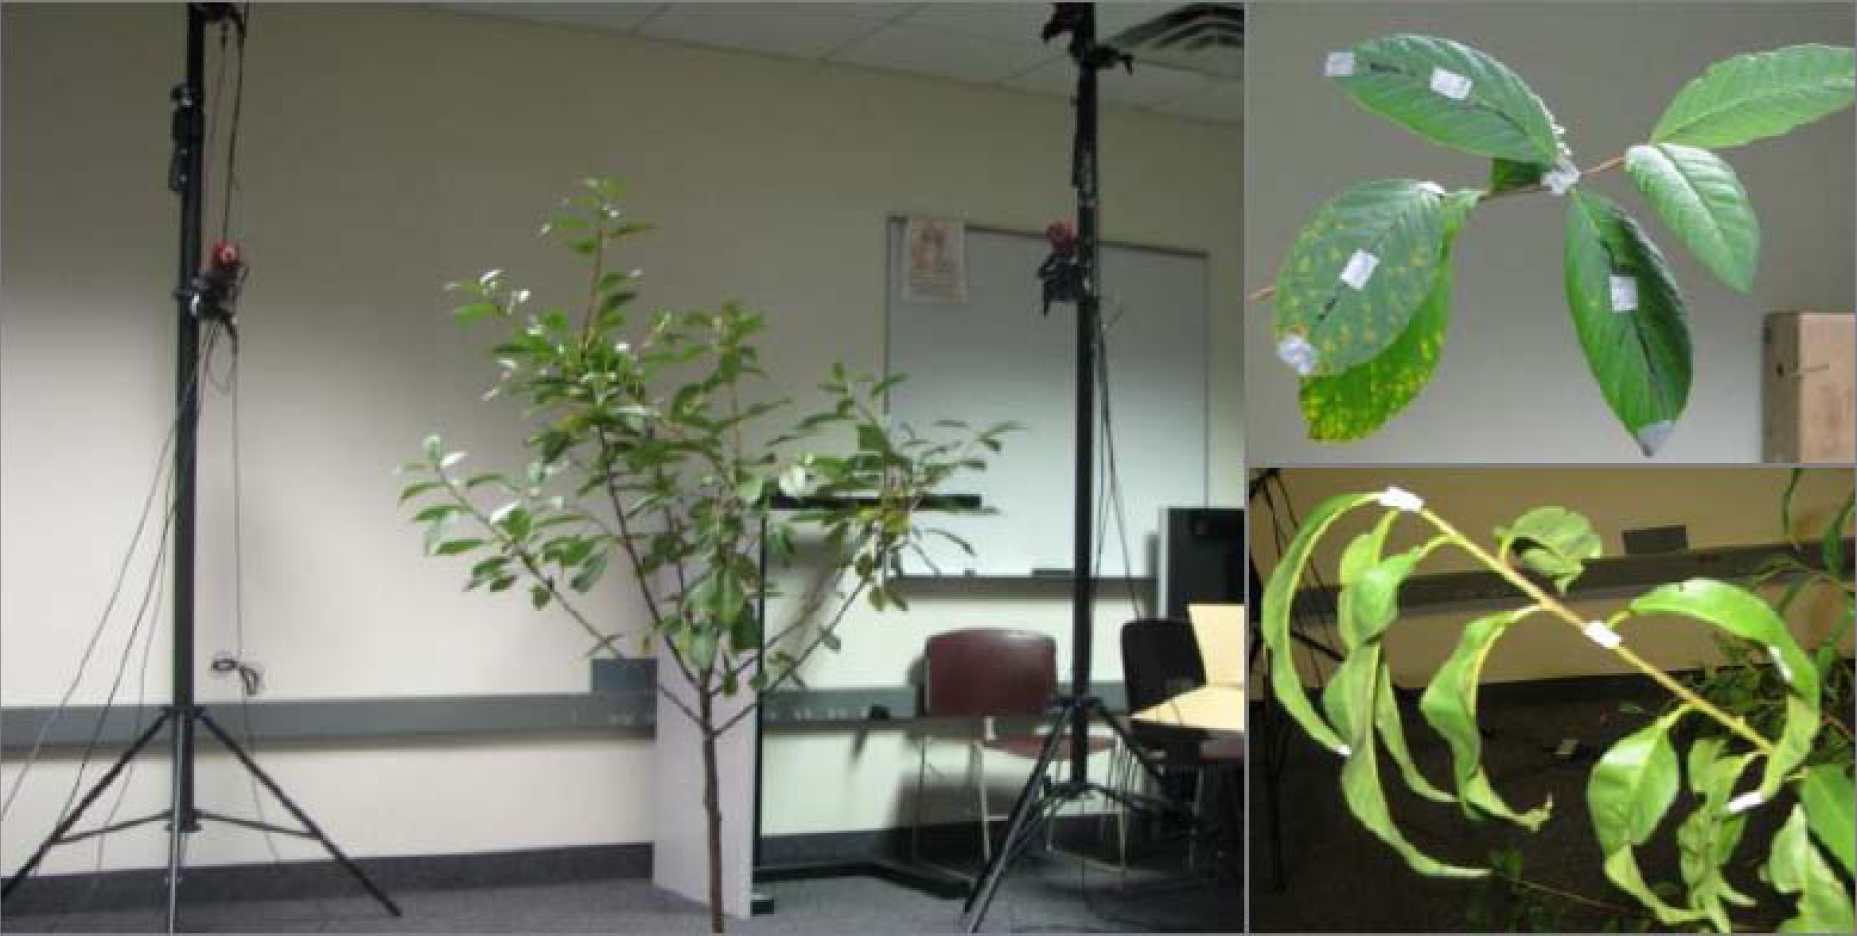
\includegraphics[width=6.0in]{experiment.PNG}
\caption[Motion capture set up for a natural tree.]{Motion capture setup for a natural tree using an optical motion capture system. }
\label{fig:Setup} 
\end{figure}

\section{Build Static Tree Geometries} 

One significant problem with motion capture of trees, compared to human performance capture, is that the branching structure, or topology, of a tree is less predictable and more complex than that of a human.  A minimal spanning tree algorithm is used with a cost function derived from motion data to create a plausible branching structure.  The branching structure is plausible when animating it with the captured motion looks plausible. The cost function is one of the contributions of this paper.  

\subsection{Skeleton and Topology Estimation} 

\begin{figure}[tb]
\centering
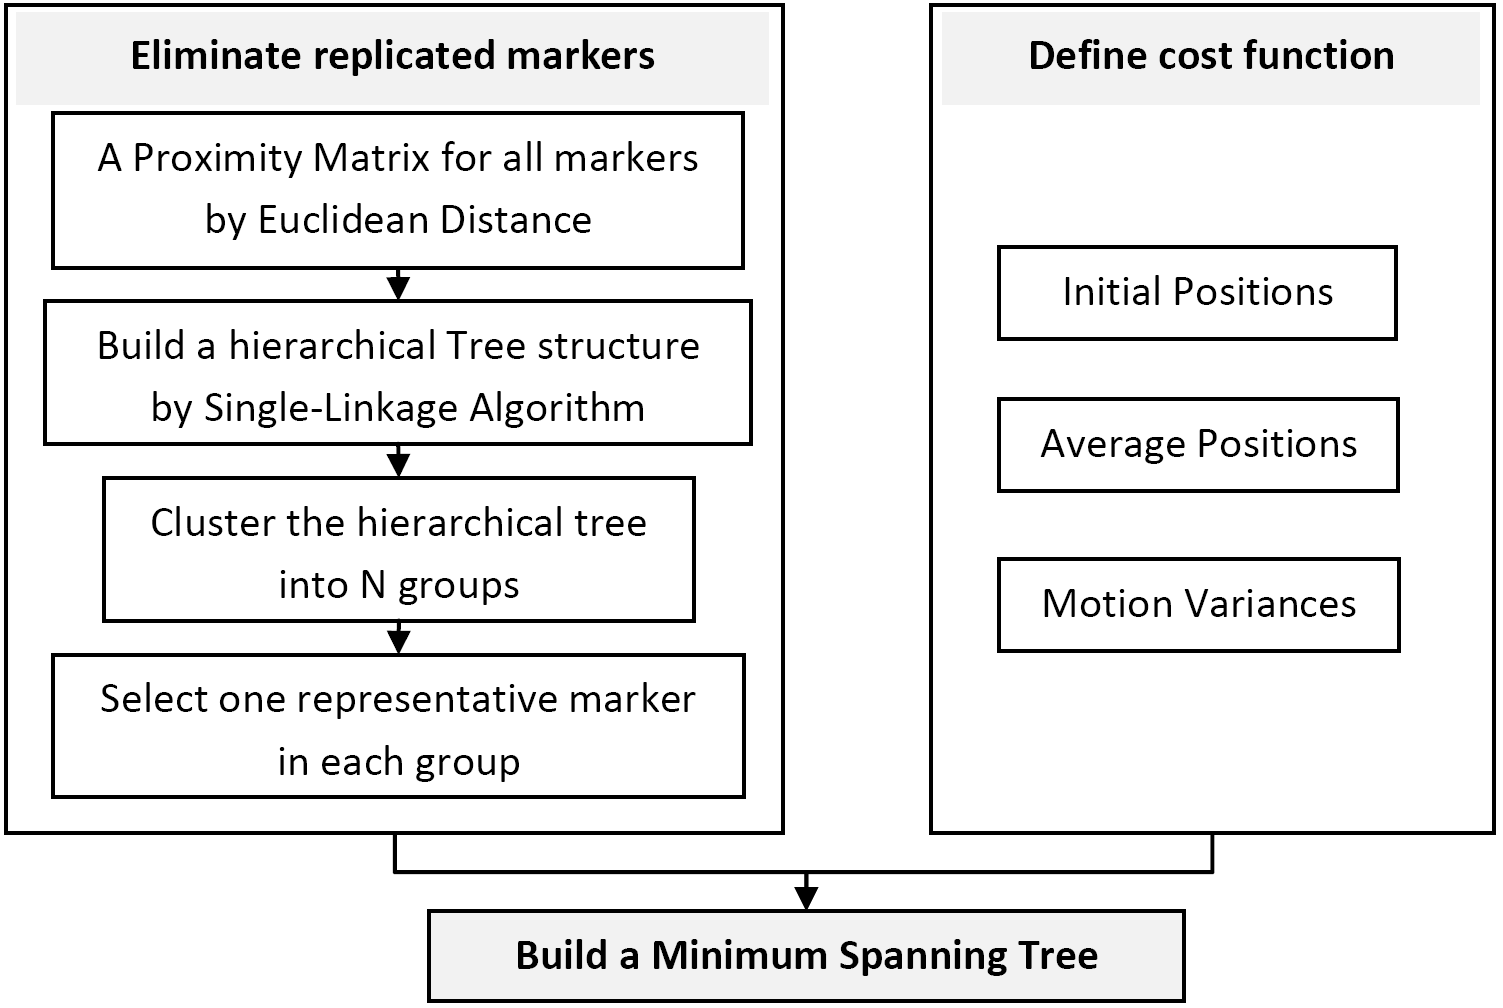
\includegraphics[width=5.0in]{skeleton.PNG}
\caption{Steps in building a tree skeleton.}
\label{fig:Skeleton} 
\end{figure}

Figure~\ref{fig:Skeleton} summarizes the process of estimating the skeleton and topology. This process has three steps. First, hierarchical clustering eliminates replicated recorded markers in each frame. Next, we use position and motion data for each marker to define a cost function.  The cost function is used to estimate the plausibility of merging two different markers. A minimum spanning tree algorithm uses a different cost function to connect the markers into a tree-like skeleton that will have plausible motion when animated using the captured motion data.

The first step, shown on the left side of Figure~\ref{fig:Skeleton}, is to eliminate duplicate, yet slightly different, recorded positions of a single marker.  We use Euclidian distance as the clustering metric. The single linkage algorithm groups markers into a hierarchy of $n$ clusters, where $n$ is the number of markers originally placed on the tree.  Within each frame, a cluster is reduced to a single representative marker.  When all frames have the correct number of markers, we further refine the representative position of each marker, either by choosing its position in the tree's rest pose or by averaging its position over time. The tree skeleton is built from the $n$ representative marker positions.  This skeleton is used for the entire capture sequence.

The second step, shown on the right side of Figure~\ref{fig:Skeleton}, computes costs for creating connections in the control skeleton between different pairs of markers based on the recorded position and motion data. Connection costs are computed for pairs of representative markers with one marker from each cluster. The cost function consists of three elements: initial position, average position over time, and variance of position over time. We assume that the branch motion is periodic. The  average position is similar to the position while the variance reflects the amplitude of the movement. The initial positions are recorded when there is no wind and the tree is stationary. The average positions are calculated as shown in the next equation in which $m$ is the number of recorded frames and $p_i$ is the 3D position for a marker at the $ith$ frame: 
\[
	   \bar{d} = \frac{1}{m}\Sigma_{i=1}^m p_i.
\]
The variance in position is similarly defined as 
\[
      \sigma^2 = \frac{1}{m}\Sigma_{i=1}^m (p_i-\bar{d})^2.
\] 

Let $\alpha$, $\beta$, and $\gamma$ be constant weighting parameters; then the cost to connect markers $M_a$ and $M_b$ is given by
\[
      \omega = \alpha||p_{M_a} - p_{M_b}|| + \beta||\bar{d}_{M_a} - \bar{d}_{M_b}|| + \gamma||\sigma_{M_a} - \sigma_{M_b}||. 
\]

The cost to connect markers $M_a$ and $M_b$ is low when $M_a$ and $M_b$ are close in both position and movement.

In the third step, we use Prim's MST algorithm with the node at the bottom of the trunk as a starting point to build the tree skeleton. Pairs of markers with similar position information and movements have low connection cost and are connected in the skeleton. This skeleton is directly taken as the input tree structure for rendering in the next step.    

Figure~\ref{fig:costResults} shows the importance of each part of the cost function. The right side of Figure~\ref{fig:costResults} shows a tree created using just the change in variance as the cost function. This cost function results in branch tips connected to branch tips because variance increases as one moves along a tree from trunk to branch tips. The middle tree was created using only positional information.  While the structure is accurate for much of the tree, several points are connected incorrectly across the middle of the tree. This will result in implausible motion when animated using the motion capture data. Using both metrics, along with average position, results in a more accurate model shown on the right.  

By combining these parameters, we connect markers with similar position and movement. For a tree with 98 clusters of markers, 66.26\% of the resulting connections are correct when compared with the actual tree. Most errors are from connecting markers in the correct branch segments but at the wrong junction points within the branch segment.   This cost function occasionally connects markers from different branches but which share close positions and movements.  In these cases, the motion of physically adjacent branch tips is similar and the resulting animation is still plausible.  

\begin{figure*}[tb]
\centering
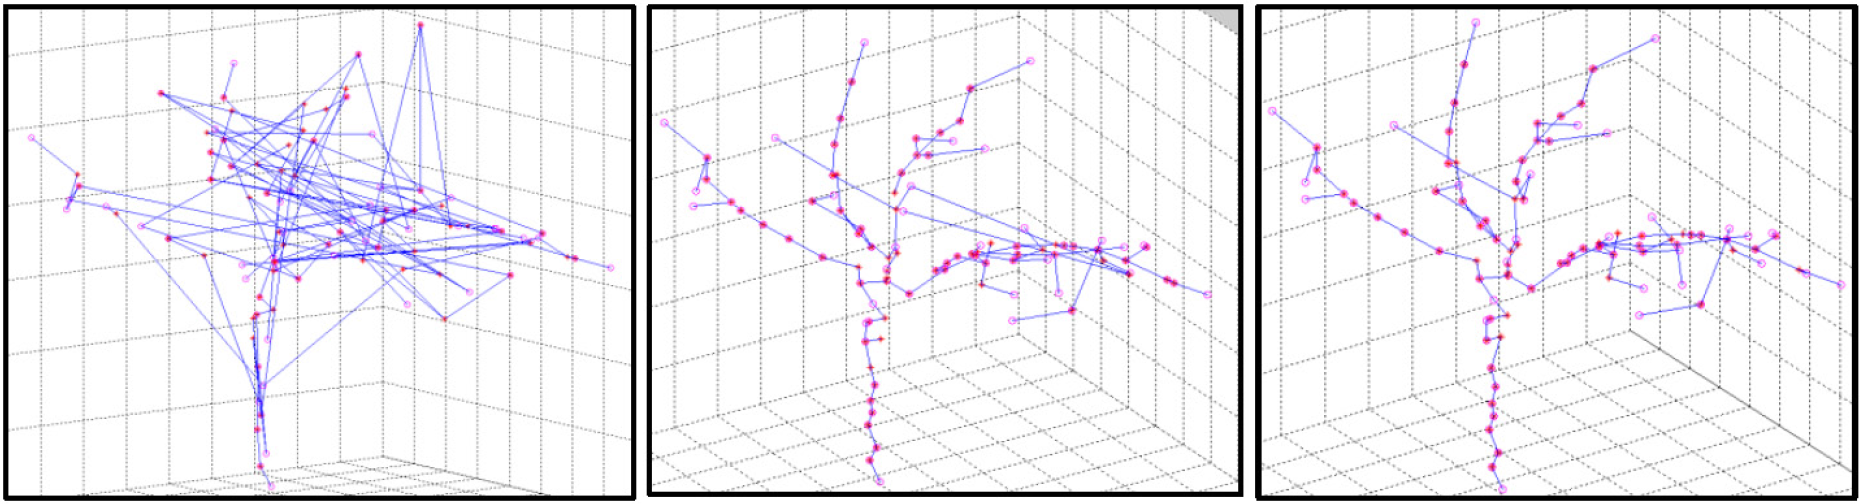
\includegraphics[width=6.0in]{cost.PNG}
\caption[Reconstructed tree topologies.]{Reconstructed tree topologies using variance, initial position, and a combination of variance, initial position, and average position.}
\label{fig:costResults} 
\end{figure*}

\subsection{Geometry of Branches and Leaves}

After the tree skeleton is created, the next step is to generate the geometric mesh. The marker points in a single branch are used as control points to create a curve. A second curve is placed at the first marker point in the branch and oriented to the first two points in the branch.  A closed circular shape is swept along the profile curve to create a NURBS surface. The profile and shape curves are discarded, leaving just the branch geometry.

Then we bind the mesh to the skeleton.  This step is separated from the previous steps so that the artist has more flexibility to modify the automatic mesh before it is bound to the skeleton. After any needed updates, the mesh is bound to the geometry. Once the geometry is bound, the artist again has the flexibility to manually tweak the binding.

Finally, a 3D point cloud inferred from photographs guides the manual placement of leaves. The leaves are placed to fill the volume occupied by the original tree. The tree volume is created using inverse volumetric rendering \cite{RecheMartinez2004} applied to 37 photographs taken from a known camera position. The resulting 3D point cloud is exported to a 3D modeling package and, after manually matching the tree skeleton with this point cloud, we manually place leaves on branches while remaining in the recorded crown volume.

\section{Build Tree Motion} 

In this section, we describe branch motion repair and leaf motion synthesis. Branch motion repair is the process of identifying and eliminating errors, gaps, and noise from the motion capture data. The resulting motion is used to animate the 3D tree model created in the prior section. 

We used the rigid body algorithm that was shipped as part of the NaturalPoint Arena software to convert unindexed point clouds into an animated skeleton. Because tree branches are non-rigid at large deflections, the resulting motion contains more gaps and errors than one might expect to find for rigid body motion capture. We use linear interpolation, a filter, and a machine learning algorithm to repair the resulting motion. The NaturalPoint Arena software provides some interpolation processes to fix motion gaps, but requires the user to manually identify gap regions and select a correction method. We automate gap detection and correction with different methods, depending on the gap size.  A machine learning based method for addressing large gaps is one of the contributions of this paper.  We use a standard curve fitting technique for small gaps. 

\subsection{Filter-based Noise Detection and Removal}

For some non-rigid motion, the rigid body motion capture system introduces anomalous artifacts to the motion signal, resulting in sporadic popping motions of certain leaves and twigs. These artifacts are detected using convolution-based filtering techniques and are replaced by fitting Bezier curves over the corresponding sections of the motion signal.  

\subsection{Small Gaps in Data}

Small gaps in data are short sequences of 100 frames or less in which no position data is recorded for a marker.  Small gaps occur when a marker becomes occluded or is otherwise lost.  Linear interpolation is used to repair small gaps because linear interpolation can be done quickly and is good enough for these gaps. 

Linear interpolation predicts missing marker positions based on the positions of neighbors. For a marker with missing position data, we find the two nearest neighbors with available position data. Then we compute Euclidean distances among the positions of these three markers and a velocity for each marker. Different distance metrics can be used. By doing linear interpolation according to the positions and velocities, we estimate the position for the missing marker. 

Linear interpolation works well if all three markers have similar movement. However, if the motions of two different, but adjacent, missing markers have their positions interpolated from the same set of nearby neighbors, the resulting interpolated motion may not preserve each marker's unique periodic motion. This may happen even though we aim to make the interpolated motion fit smoothly with the existing motion for each marker. However, losing periodic movements for a short period of time when repairing a small gap still results in visually plausible motion. 

\subsection{Large Gaps in Data}

Repairing large gaps in data is done using a more sophisticated interpolation scheme so that the synthesized motion has good periodic properties.  Large gaps in data refer to gaps which comprise more than 40\% of the entire motion trace collected for a single marker. A machine learning algorithm builds a function that is used to infer motion that is used to fill large gaps.  

Given the connection between two adjacent markers, motion data for both markers at low wind speed, and motion data for one marker at high speed, the machine learning algorithm trains a support vector machine (SVM) and defines a correlation function. This approach is based on the observation that good data is captured for all markers at low wind speed, but large gaps appear in the data for some markers at high wind speed.  The SVM learns a correlation between data from two markers collected at low wind speeds.  This relationship is used to estimate missing motion at high wind speeds under the assumption that the relationship is not sensitive to wind velocity.

The tree skeleton structure is used to find the nearest topological neighbor with motion data for both high and low speeds. In most cases, markers at branch tips have missing data while markers at the branch base have the required data. This is because markers at the branch base move more rigidly than markers on tips. In these cases, the marker at a tip has large gaps in motion data and its nearest neighbor in the direction of the branch base often lies on the same branch.

Sequential minimal optimization (SMO) \cite{keerthi:nc01,platt:mit99} trains an SVM, which defines the correlation function between the two markers' positions at low speed. In order to improve the precision of the correlation function and to avoid phase differences, the motion data from each series is sorted in ascending order of displacement. Let $M_a$ be the nearest neighbor to $M_b$, which is a marker with missing motion at high speed. $M_a$ and $M_b$ both have motion data at low speed.  A learned function $F$ estimates the position of $M_b$ given $M_a$. Position data from $M_a$ recorded at high wind speeds is given to $F$, which then estimates $M_b$'s position at high wind speeds.  

Figure~\ref{fig:result_curve} shows the estimated and actual position for one marker at low and high wind speeds. The vertical axis is the displacement and the horizontal axis is the frame number. In this figure, the motion of marker $M_a$ at low wind speed, which is the topmost trace on the left, is used with the recorded motion of marker $M_b$, which is the lower trace on the left, to learn a function that predicts the position of $M_b$ given the position of $M_a$.  For comparison, we placed the predicted position of $M_b$ on the graph as well.  The predicted position of $M_b$ closely matches the actual position at low wind speeds.  At high wind speeds, shown on the right, we held back the recorded position of $M_b$ and predicted the position of $M_b$ in each frame given only the position of $M_a$.  The predicted position of $M_b$ at high speeds closely matches the actual position of $M_b$ but tends to overestimate the amount of displacement in $M_b$. 

\begin{figure}[ht]
\centering
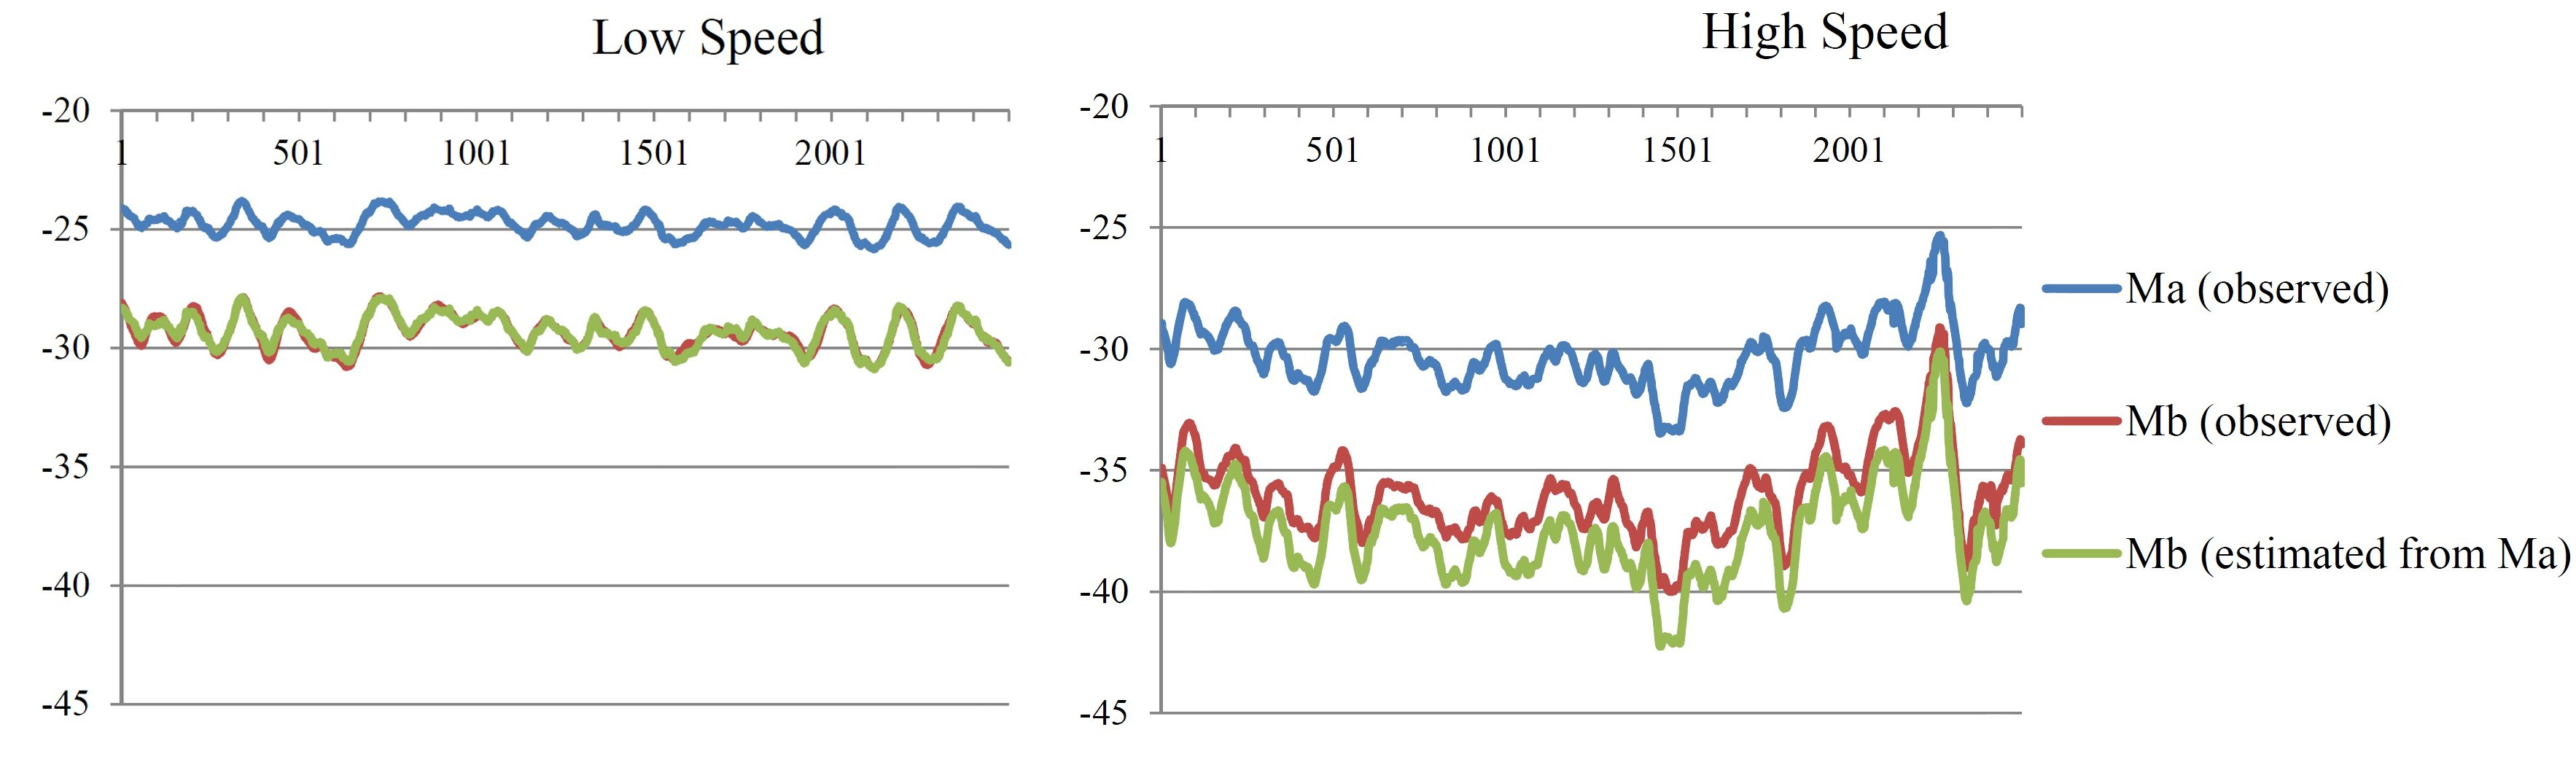
\includegraphics[width=6.0in]{low-speed-high-speed.jpg}
\caption[Predicted versus actual displacement.]{Predicted versus actual displacement for a marker at low and high wind speeds.}
\label{fig:result_curve} 
\end{figure}

\subsection{ Leaf Motions}

Motion data applied to leaves is based on motion captured from only a few leaves. This motion is scaled and offset to simulate a greater variety and randomness of leaf motion. The leaf geometry deforms along motion curves applied at the end, at the middle, and near the stem.

The complexity of leaves moving in the wind precludes any attempt to correlate leaf movement with the movement of the branch it is on. Leaves can be quite turbulent or almost still on a branch that is either very still or sweeping any position through its arcs of movement. However, motion of the leaves is scaled with the branch motion to suggest that they are driven by the same wind. These two motion sets can also be decoupled for an artist to achieve a particular effect. 

%\input{conclusion.tex} 
\section{Results} 

The final animation is shown in the video that accompanies this paper. In that video, most motion capture artifacts have been removed and the motion looks reasonable.  Results in skeleton estimation and motion repair, which are the main contributions of this paper, were given in the preceding sections.

%\input{futurework.tex} 
\section{Conclusion and Future Work} 

A plausible tree skeleton can be reconstructed using a minimal spanning tree algorithm over a cost function defined using position and motion data.  The skeleton is plausible in the sense that replaying the capture motion on the skeleton looks realistic.  Gaps and errors in motion capture data for trees can be replaced with data interpolated from neighboring branch motion.  These are important steps toward realizing motion capture of trees for tree animation in games.  Motion capture of tree motion is a good match for motion in games because the resulting motion is realistic but requires only replaying, rather than simulating, actual motion.  

We had hoped to get better results with the repaired data and the rigid body algorithm we used. Based on these results, we believe that investigating other approaches to processing the point cloud are more promising than repairing the errors caused by using the rigid body algorithm we used.  

Future work could take several interesting directions. One of these is to avoid defining rigid bodies for each branch while capturing motion by defining the tree as a non-rigid body, which is a truer representation of its natural form. More work needs to be done to be sure the algorithm scales well for capturing the motion of other tree subjects as well as for transferring captured motion from one tree to another. By capturing data from multiple trees at once, the interactions among them could be studied and applied to simulate groups of trees or even forests.